
\section{Mobile App}

    \subsection{Overview}
The mobile app is used to visualize 3D models, accessing files from the website and scanning QR codes. It is an Android application using ARCore, Google's newest Augmented Reality library.
    \subsection{Technologies Used}
The Android app is developed in Android Studio, primarily with the Java programming language. The following libraries were used in this project.
    \begin{itemize}
        \item ARCore - Support for AR on Android devices (off of the Google Play Store)
        \begin{itemize}
            \item Only works on specific devices (as of 4/26/2018)
            \item Use OpenGL to draw models, ARCore only performs tracking/world mapping
        \end{itemize}
        \item Obj Parser
        \begin{itemize}
            \item Used by the example AR Core application to draw the model
            \item Parses the obj files
            % \item \url{https://github.com/JohnLXiang/arcore-sandbox}
        \end{itemize}
        \item QR Code Reader - included in Android project dependencies
        \item Volley - Google library for network communications between app and website
        \item Room - Google library that provides an abstraction layer over SQLite for storing file listings in the phone's database.
    \end{itemize}

    \subsection{Data Flow}

    \begin{figure}[H]
        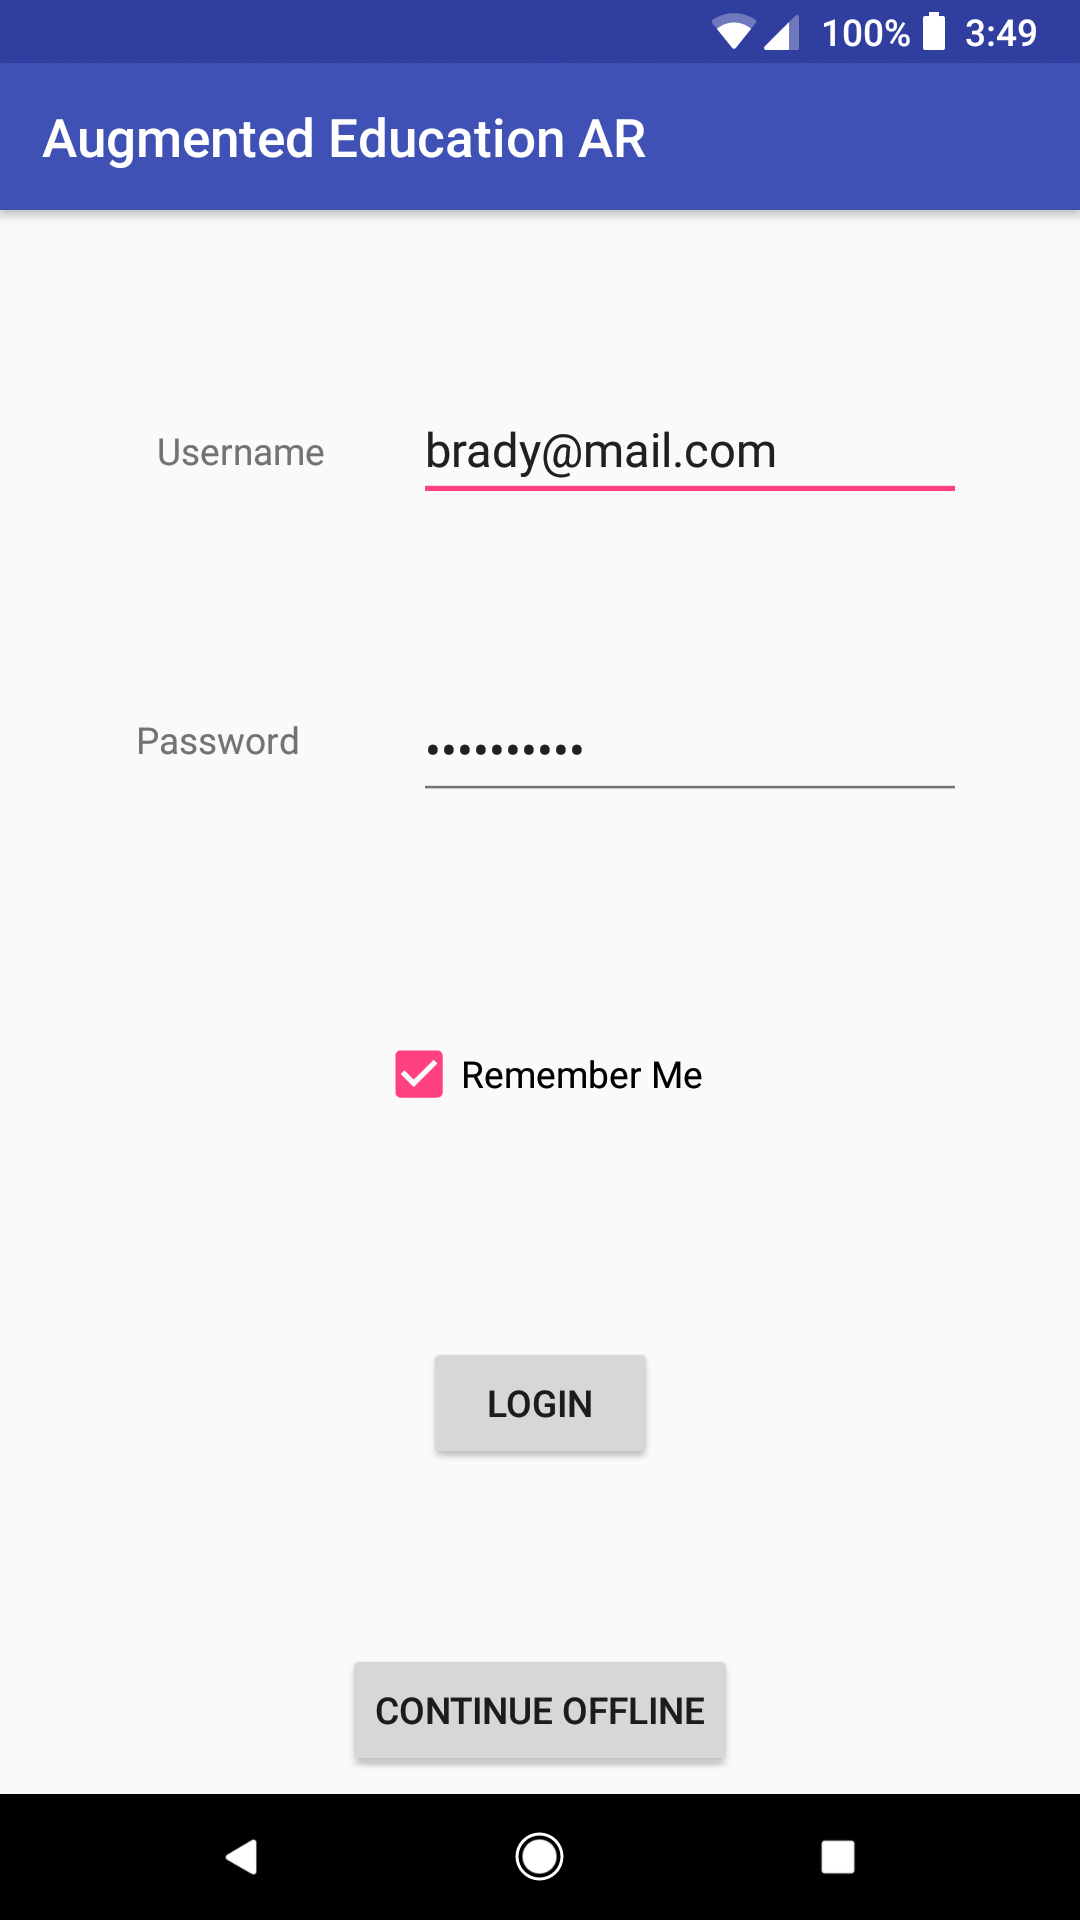
\includegraphics[width=0.5\textwidth]{Mobile/Mobile_MainActivity}
        \centering
        \caption{Mobile App - Login}
        \label{fig:mobileLoginActivity}
    \end{figure}

    \begin{figure}[H]
        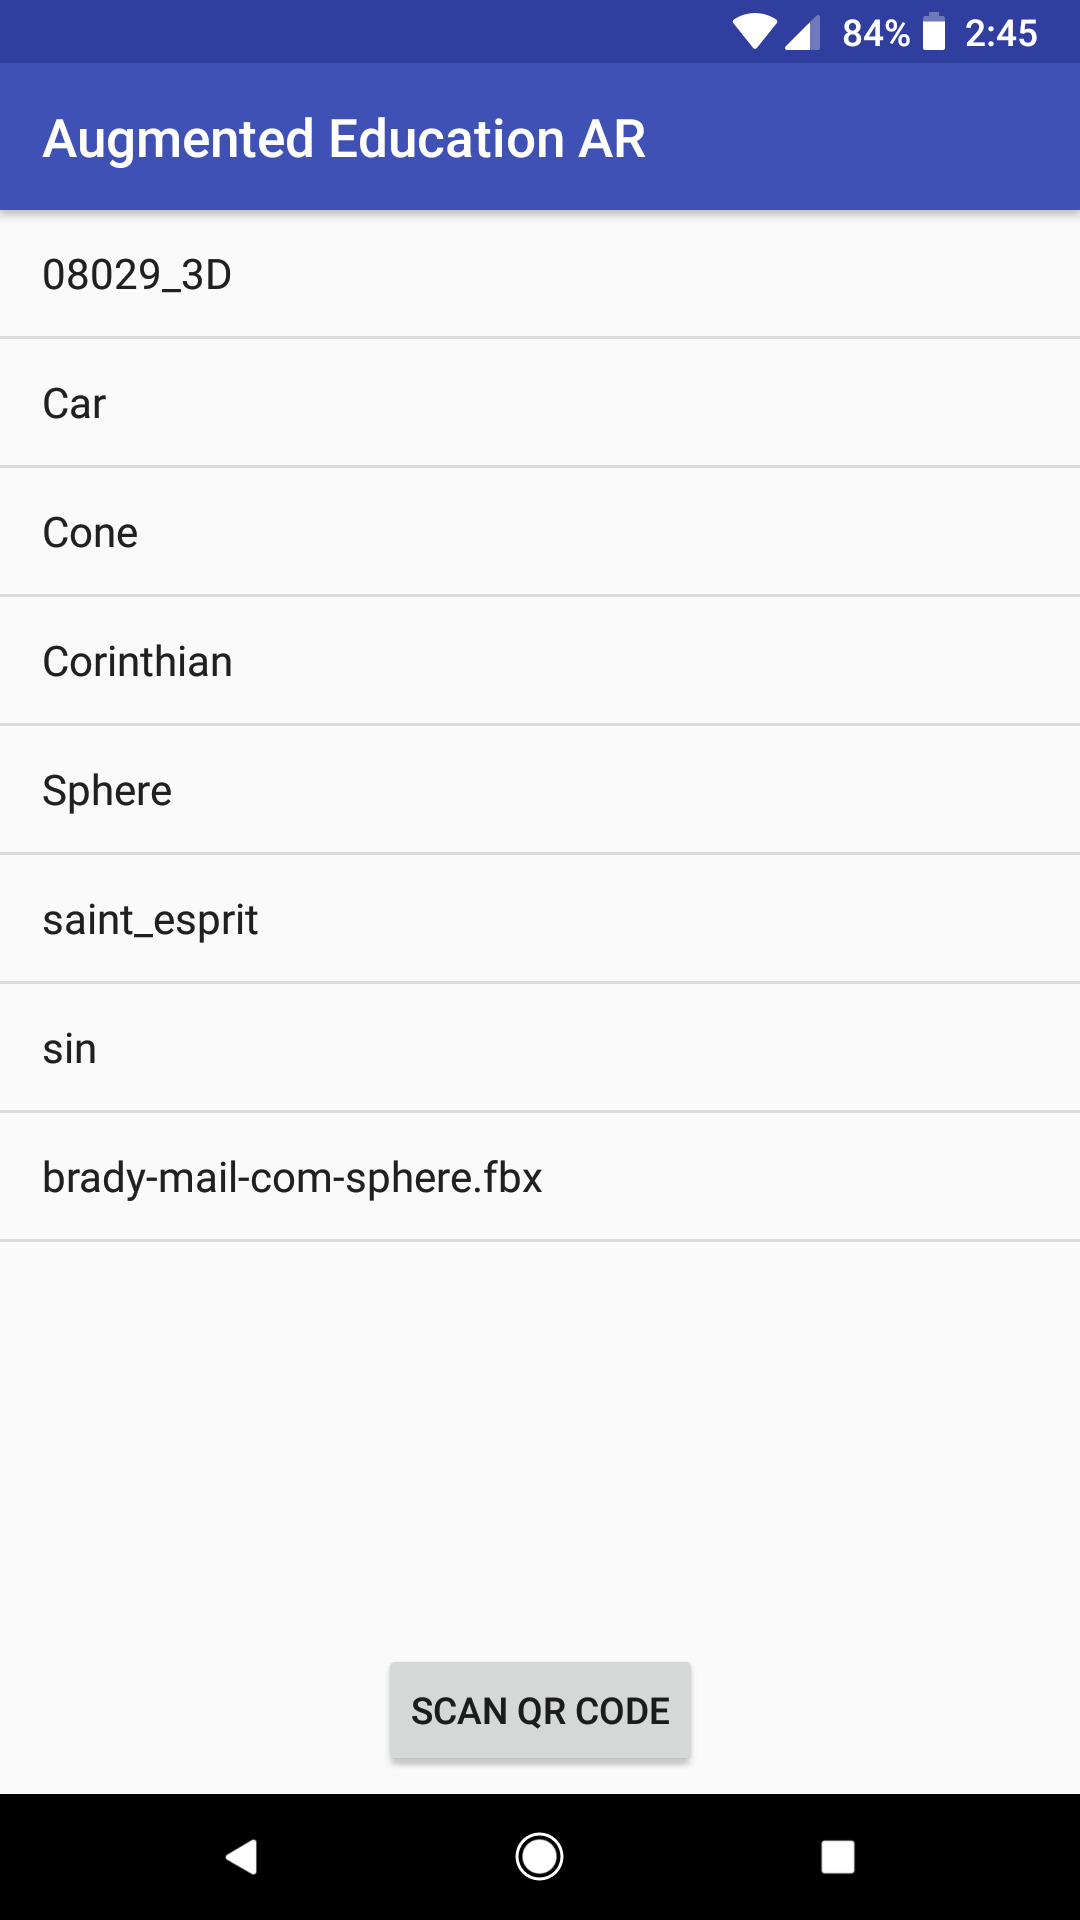
\includegraphics[width=0.5\textwidth]{Mobile/Mobile_ModelList}
        \centering
        \caption{Mobile App - Model Listing}
        \label{fig:mobileModelList}
    \end{figure}

    \begin{figure}[H]
        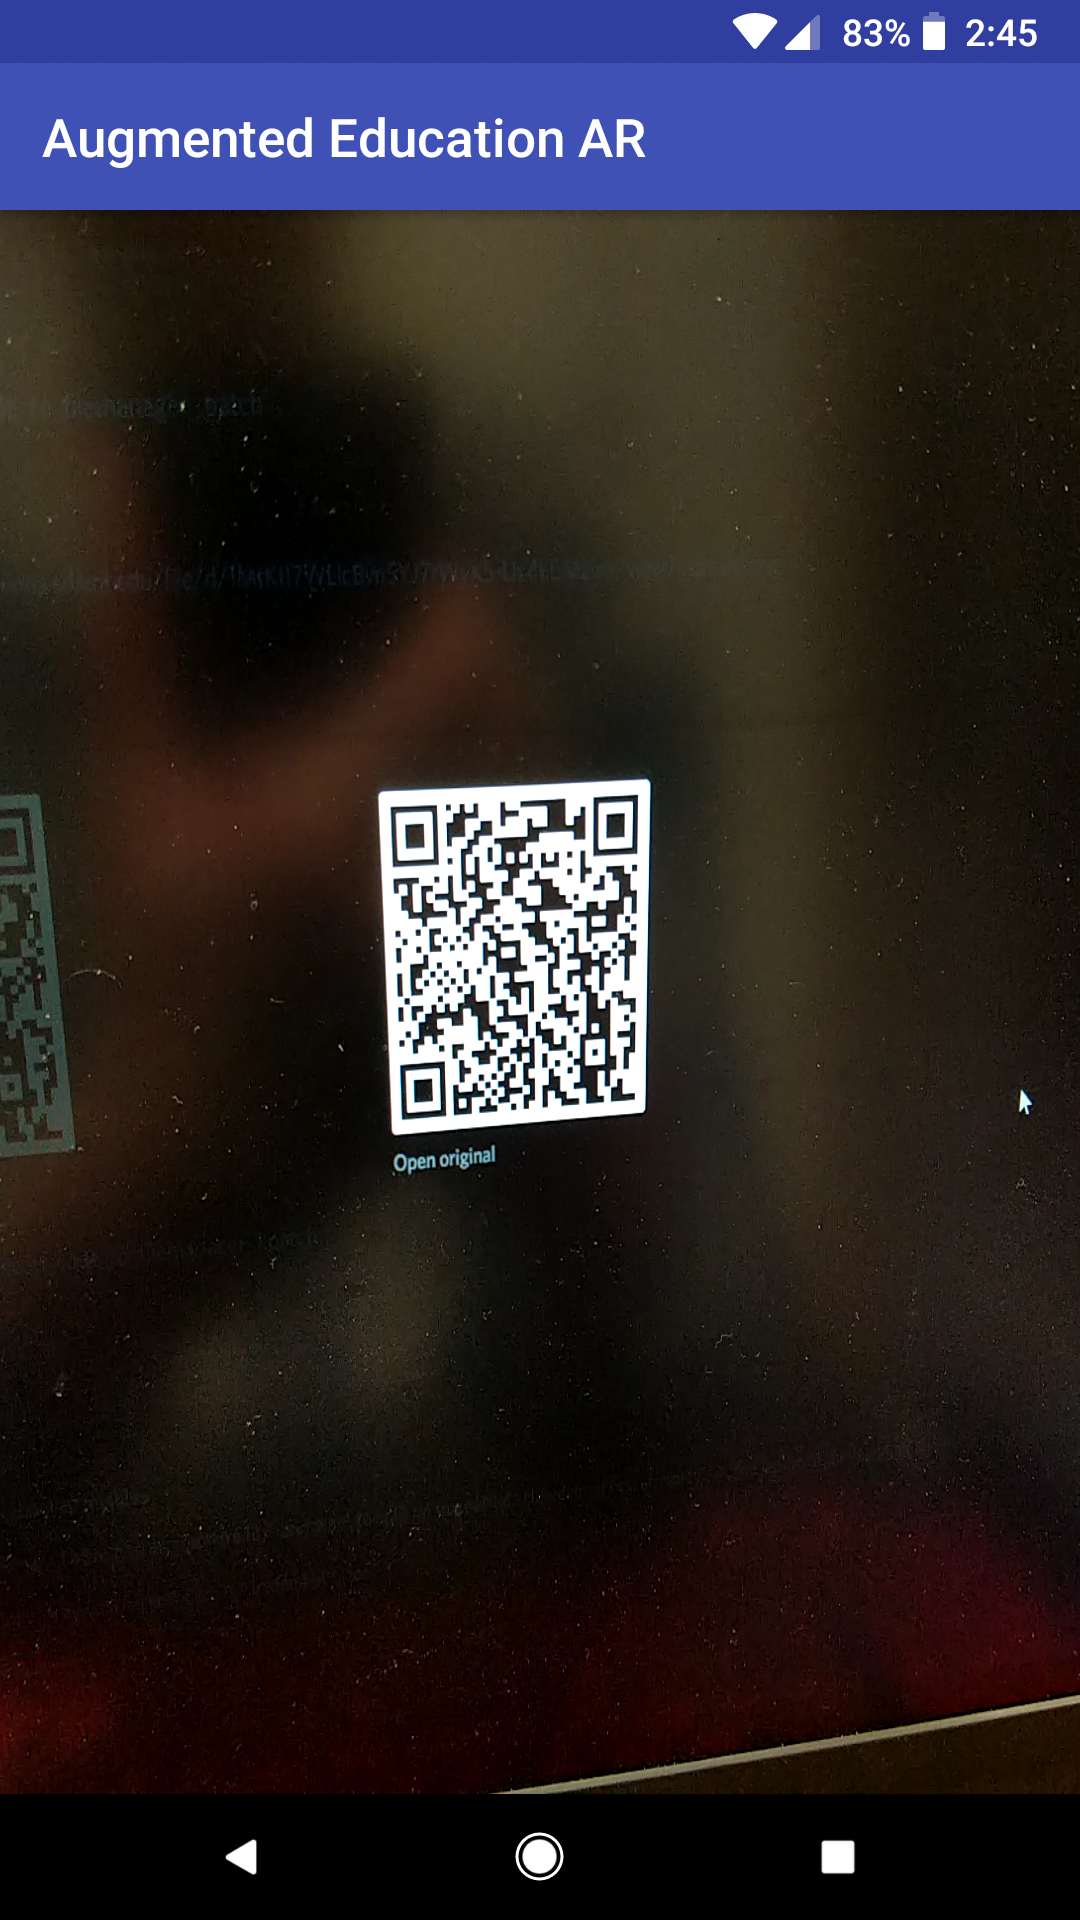
\includegraphics[width=0.5\textwidth]{Mobile/Mobile_QRScanning}
        \centering
        \caption{Mobile App - QR Code Scanning}
        \label{fig:mobileQRScanning}
    \end{figure}

    \begin{figure}[H]
        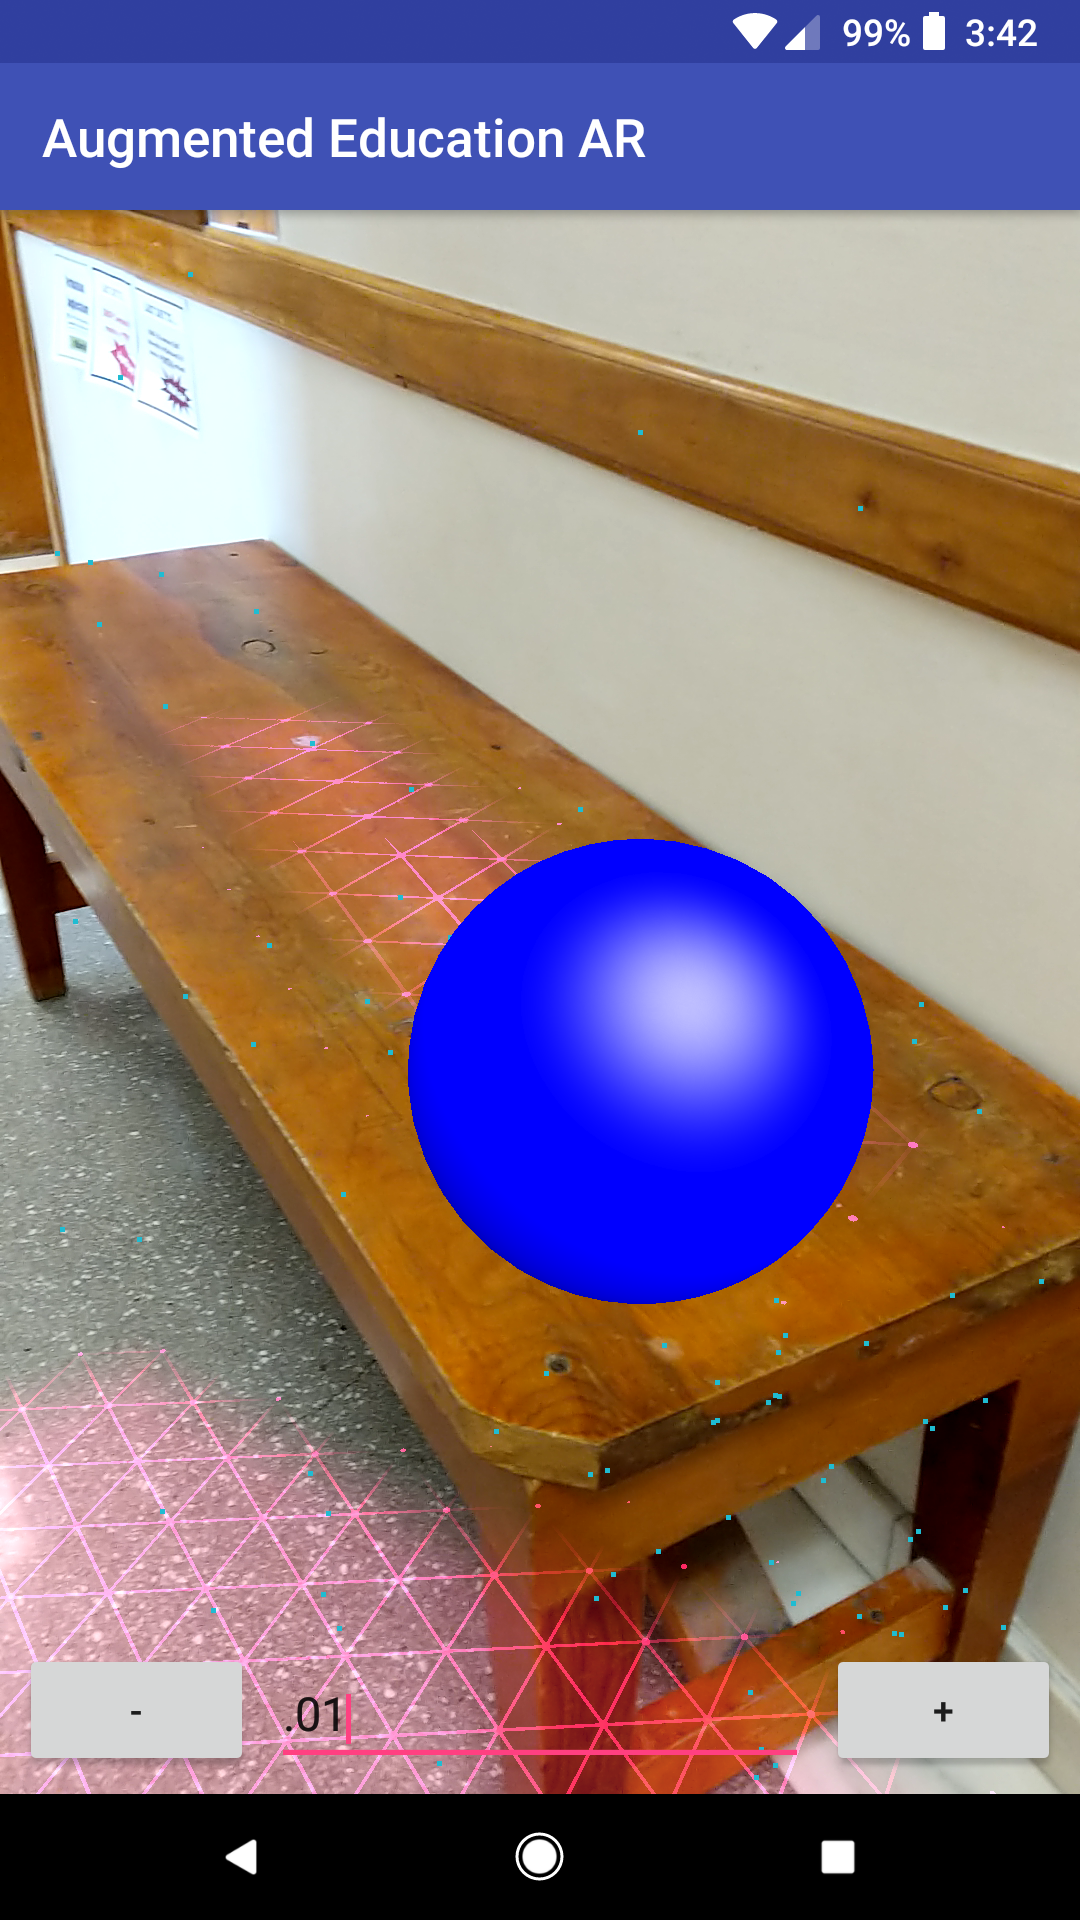
\includegraphics[width=0.5\textwidth]{Mobile/Mobile_BlueSphere}
        \centering
        \caption{Mobile App - Model Viewer}
        \label{fig:mobileModelViewer}
    \end{figure}

    \subsection{Design Details}

        \subsubsection{Overview}
The mobile app software is written in Android Studio in the Java programming language. It is an object oriented program with "activities" being the different screens that users can move between. The app has four main screens which are the login, file listing, QR code reader, and AR viewer.
        \subsubsection{Code Structure}


    